\documentclass{article}

\usepackage{graphicx}
\usepackage{subcaption}
\usepackage{amsmath}
\usepackage{float}
\usepackage{listings}
\usepackage{xcolor}
\usepackage{float}

\lstset{
    language=C++,
    basicstyle=\ttfamily\footnotesize,
    breaklines=true,
    numbers=left,
    stepnumber=1,
    numbersep=5pt,
    showspaces=false,
    showstringspaces=false,
    tabsize=2
}

\title{Ampliando e Reduzindo Imagens por Interpolação Bilinear\\ Projeto 01-2024.2: Gp. 1}
\author{André Filipe de Medeiros - 542104\\ Ryan Erik Lima da Silva - 542103}
\date{\today}

\begin{document}
\maketitle

\newpage
\section{Resumo}
O presente relatório descreve a implementação de um programa em C++ para ampliar e reduzir imagens com interpolação bilinear. Esse método calcula os valores dos pixels em uma nova resolução com base nos quatro vizinhos mais próximos. O programa permite redimensionar uma imagem de acordo com a resolução desejada (em dpi). 
Durante a atividade, reduziu-se imagem de 1250 dpi para 100 dpi e, em seguida, ampliou-se de volta para 1250 dpi, observando a perda de qualidade. O programa também foi aplicado em outras imagens, demonstrando a eficácia da técnica na ampliação e redução de imagens.

\section{Discussão Técnica}

\subsection{DPI}
Pontos por polegadas (dpi) é uma unidade de resolução comumente utilizada em imagens digitais. Essa grandeza indica a quantidade de pixels que existem em uma área de uma polegada quadrada. Em geral, quanto maior for o dpi de uma imagem, maior será sua nitidez. Assim, o dpi é um fator importante para a qualidade da imagem. A razão de dpis é 
utilizada na mudança de resolução de uma imagem, seu valor é calculado por:

\begin{equation}
    r  = \frac{DPI_{1}}{DPI_{2}}
\end{equation}

Em que, $r$ é a razão de dpis, $DPI_{1}$ é a dpi original e $DPI_2$ é a dpi desejada.

\subsection{Interpolação Bilinear}
A interpolação bilinear é um método para redimensionamento de imagens. Esse método estima o valor de um pixel em uma nova posição com base nos quatro pixels vizinhos mais próximos, utilizando uma média ponderada das distâncias horizontais e verticais. Embora seja mais precisa que métodos simples, como a interpolação por vizinho mais próximo, a bilinear pode introduzir artefatos, como suavização excessiva ou perda de detalhes, especialmente ao ampliar excessivamente uma imagem. A fórmula da interpolação bilinear para calcular o valor \( f(x, y) \) é dada por:

\begin{equation}
f(x, y) = \frac{
    (x_2 - x) \cdot (y_2 - y) \cdot f(x_1, y_1) + 
    (x - x_1) \cdot (y_2 - y) \cdot f(x_2, y_1) 
}{(x_2 - x_1) \cdot (y_2 - y_1)} + 
\end{equation}
\[
\frac{
    (x_2 - x) \cdot (y - y_1) \cdot f(x_1, y_2) + 
    (x - x_1) \cdot (y - y_1) \cdot f(x_2, y_2)
}{(x_2 - x_1) \cdot (y_2 - y_1)}
\]

Onde:\( f(x_1, y_1), f(x_2, y_1), f(x_1, y_2), f(x_2, y_2) \) são os valores dos pixels nos quatro pontos mais próximos. \( (x_1, y_1), (x_2, y_2) \) são as coordenadas dos quatro pixels vizinhos mais próximos ao ponto \( (x, y) \).
\( (x, y) \) são as coordenadas do pixel que estamos calculando na nova imagem (redimensionada).

\section{Discussão dos Resultados}

Após a escrita do \textit{script} em C++ que amplia e reduz (em dpi) uma imagem através de interpolação bilinear, submetemos a Figura \ref{fig:clock_original}
a uma redução de 1250 dpi a 100 dpi e chegamos à Figura \ref{fig:clock_300dpi}. Depois, através de interpolação bilinear, ampliamos de volta a Figura \ref{fig:clock_300dpi}
de 100 dpi a 1250 dpi e a Figura \ref{fig:clock_1250dpi} é o resultado.

\begin{figure}[H]
    \centering
    \caption{Imagens do relógio.}
    \begin{subfigure}[b]{0.3\textwidth}
        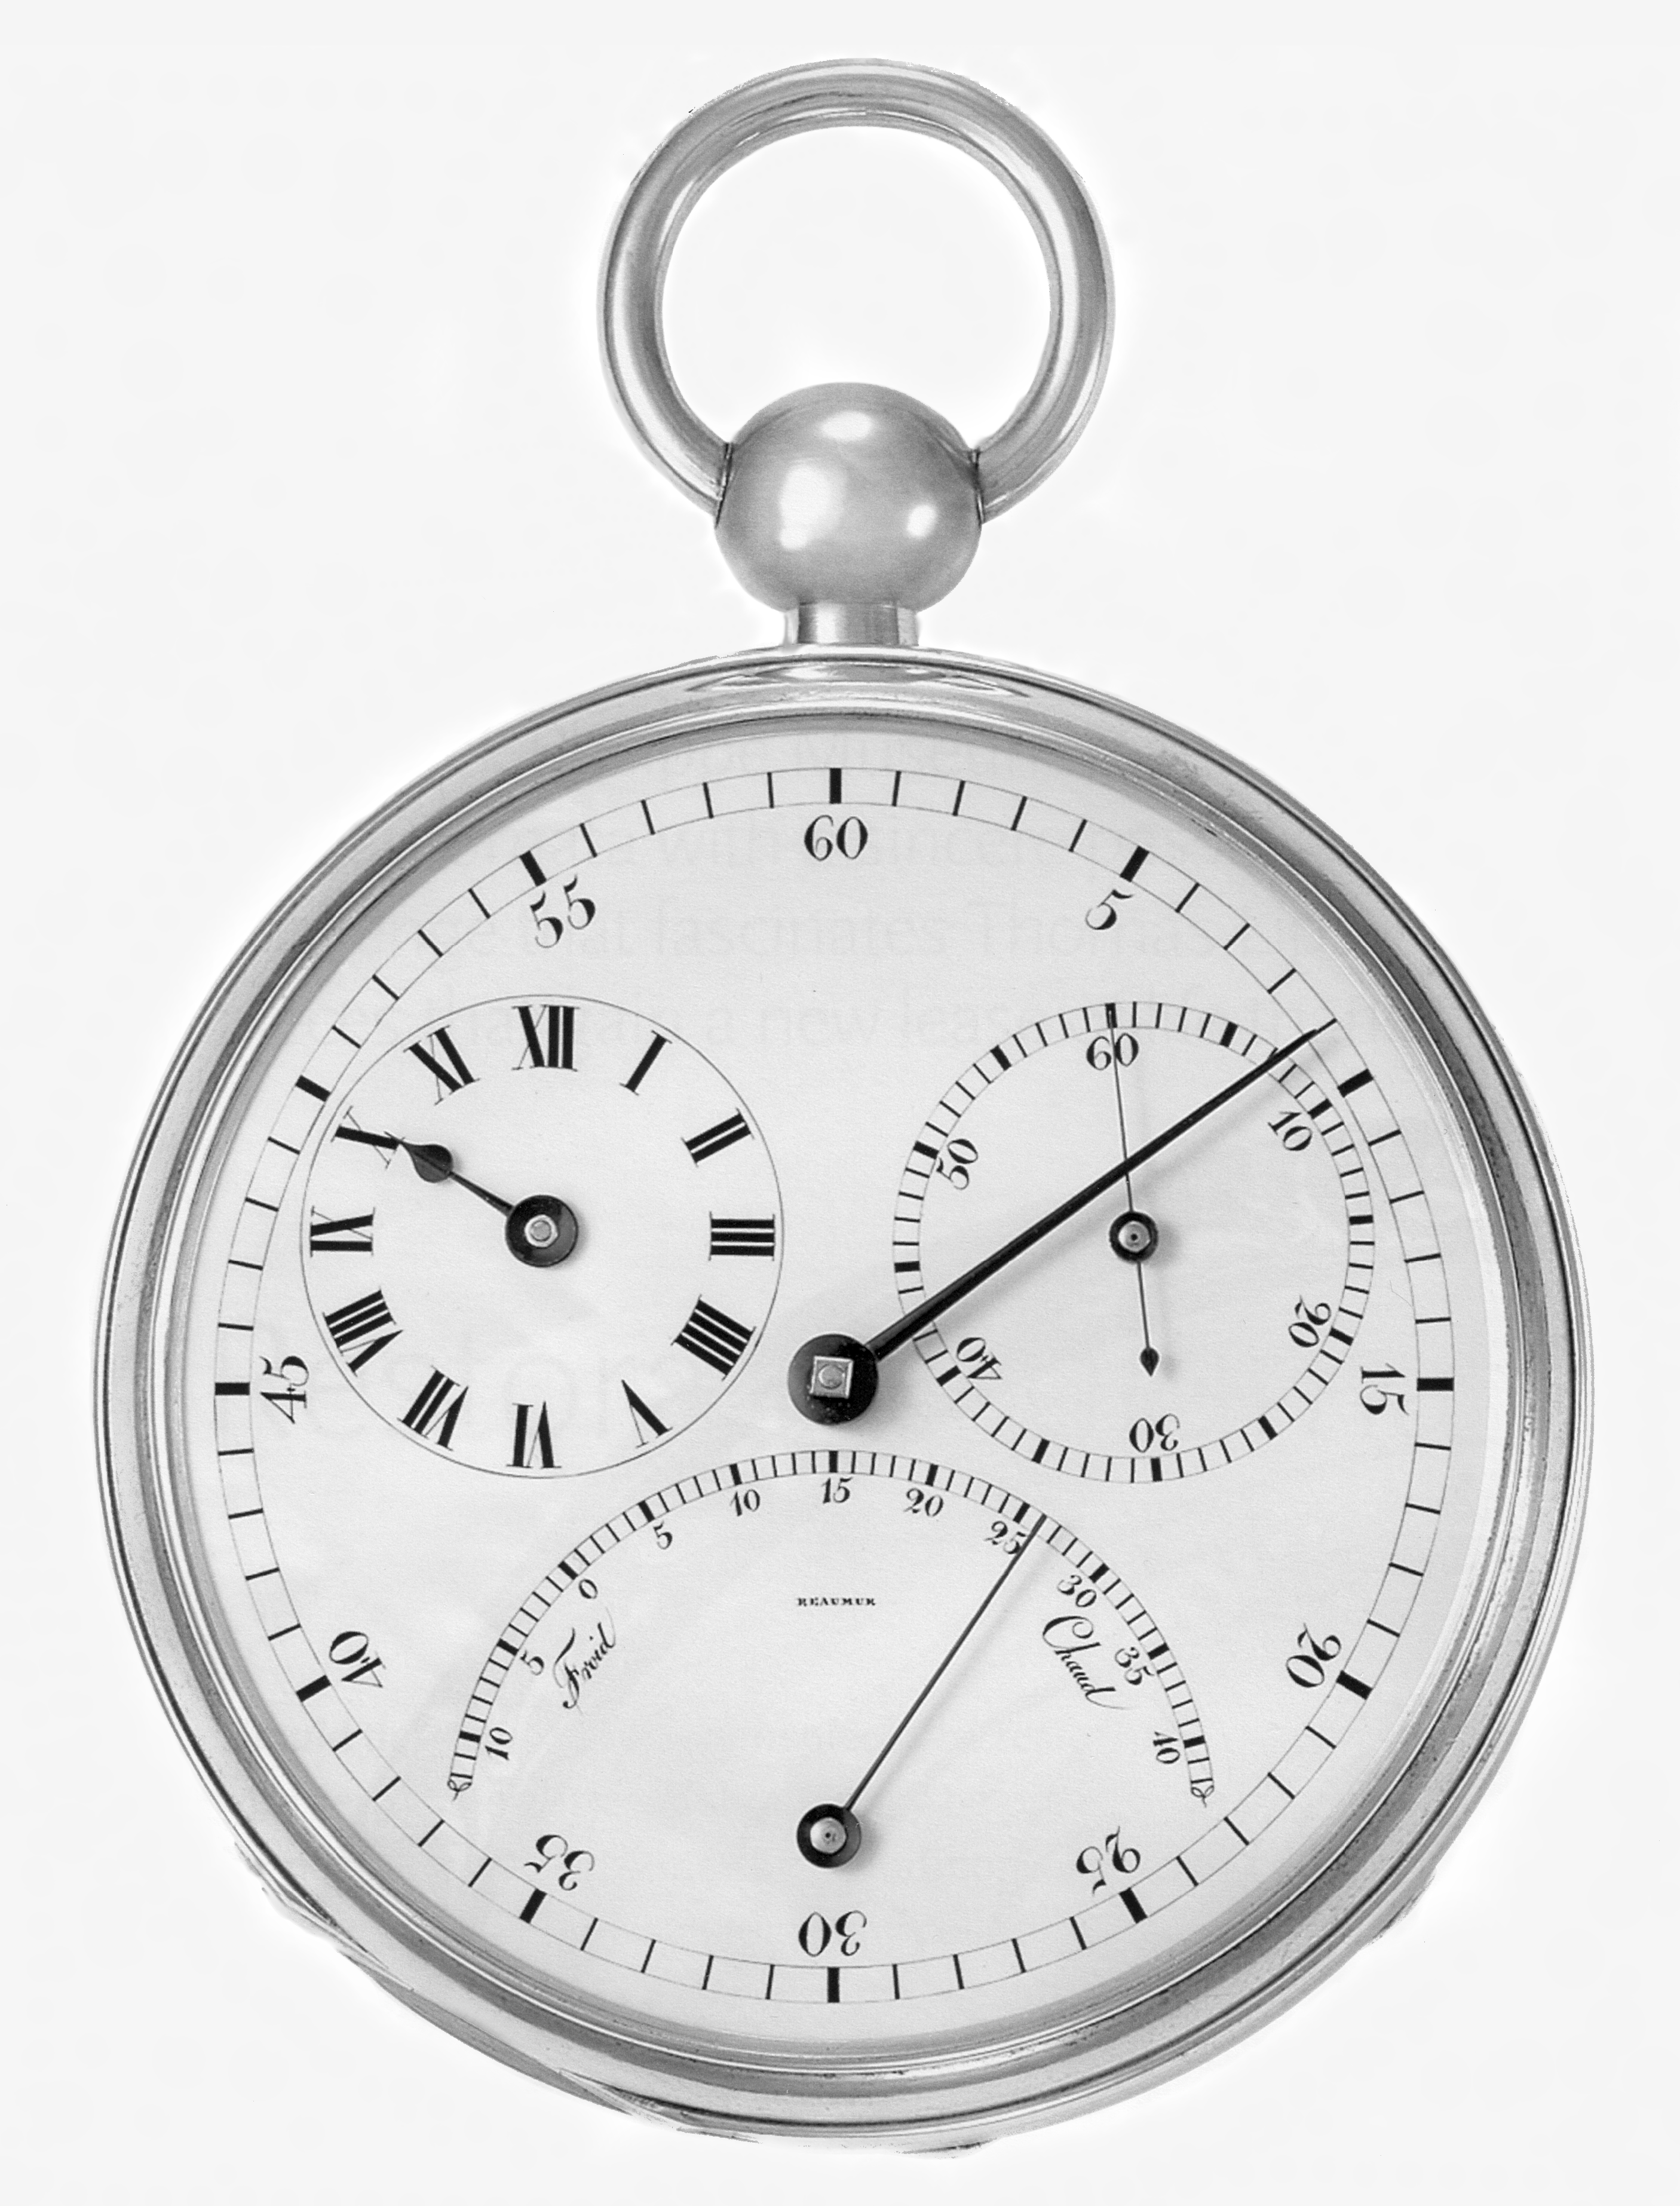
\includegraphics[width=\textwidth]{imgs/1.png}
        \caption{Imagem original 1250 dpi.}
        \label{fig:clock_original}
    \end{subfigure}%
    \hfill
    \begin{subfigure}[b]{0.3\textwidth}
        \includegraphics[width=\textwidth]{imgs/2.png}
        \caption{Imagem modificada com 100 dpi.}
        \label{fig:clock_300dpi}
    \end{subfigure}%
    \hfill
    \begin{subfigure}[b]{0.3\textwidth}
        \includegraphics[width=\textwidth]{imgs/3.png}
        \caption{Imagem modificada com 1250 dpi.}
        \label{fig:clock_1250dpi}
    \end{subfigure}
    \label{fig:clock_comparison}
\end{figure}

Percebe-se que houve uma redução de nitidez quanto se reduziu a imagem de 1250 a 100 dpi.
Após aplicação da interpolação de 100 a 1250 dpi, percebe-se uma suavização na intensidade dos pixels da imagem.

Com a diferença entre as imagens, percebe-se a perca de informação após a redução de dpi em relação à imagem original.
\begin{figure}[H]
    \centering
    \caption{Imagens diferença do relógio.}
    \begin{subfigure}[b]{0.3\textwidth}
        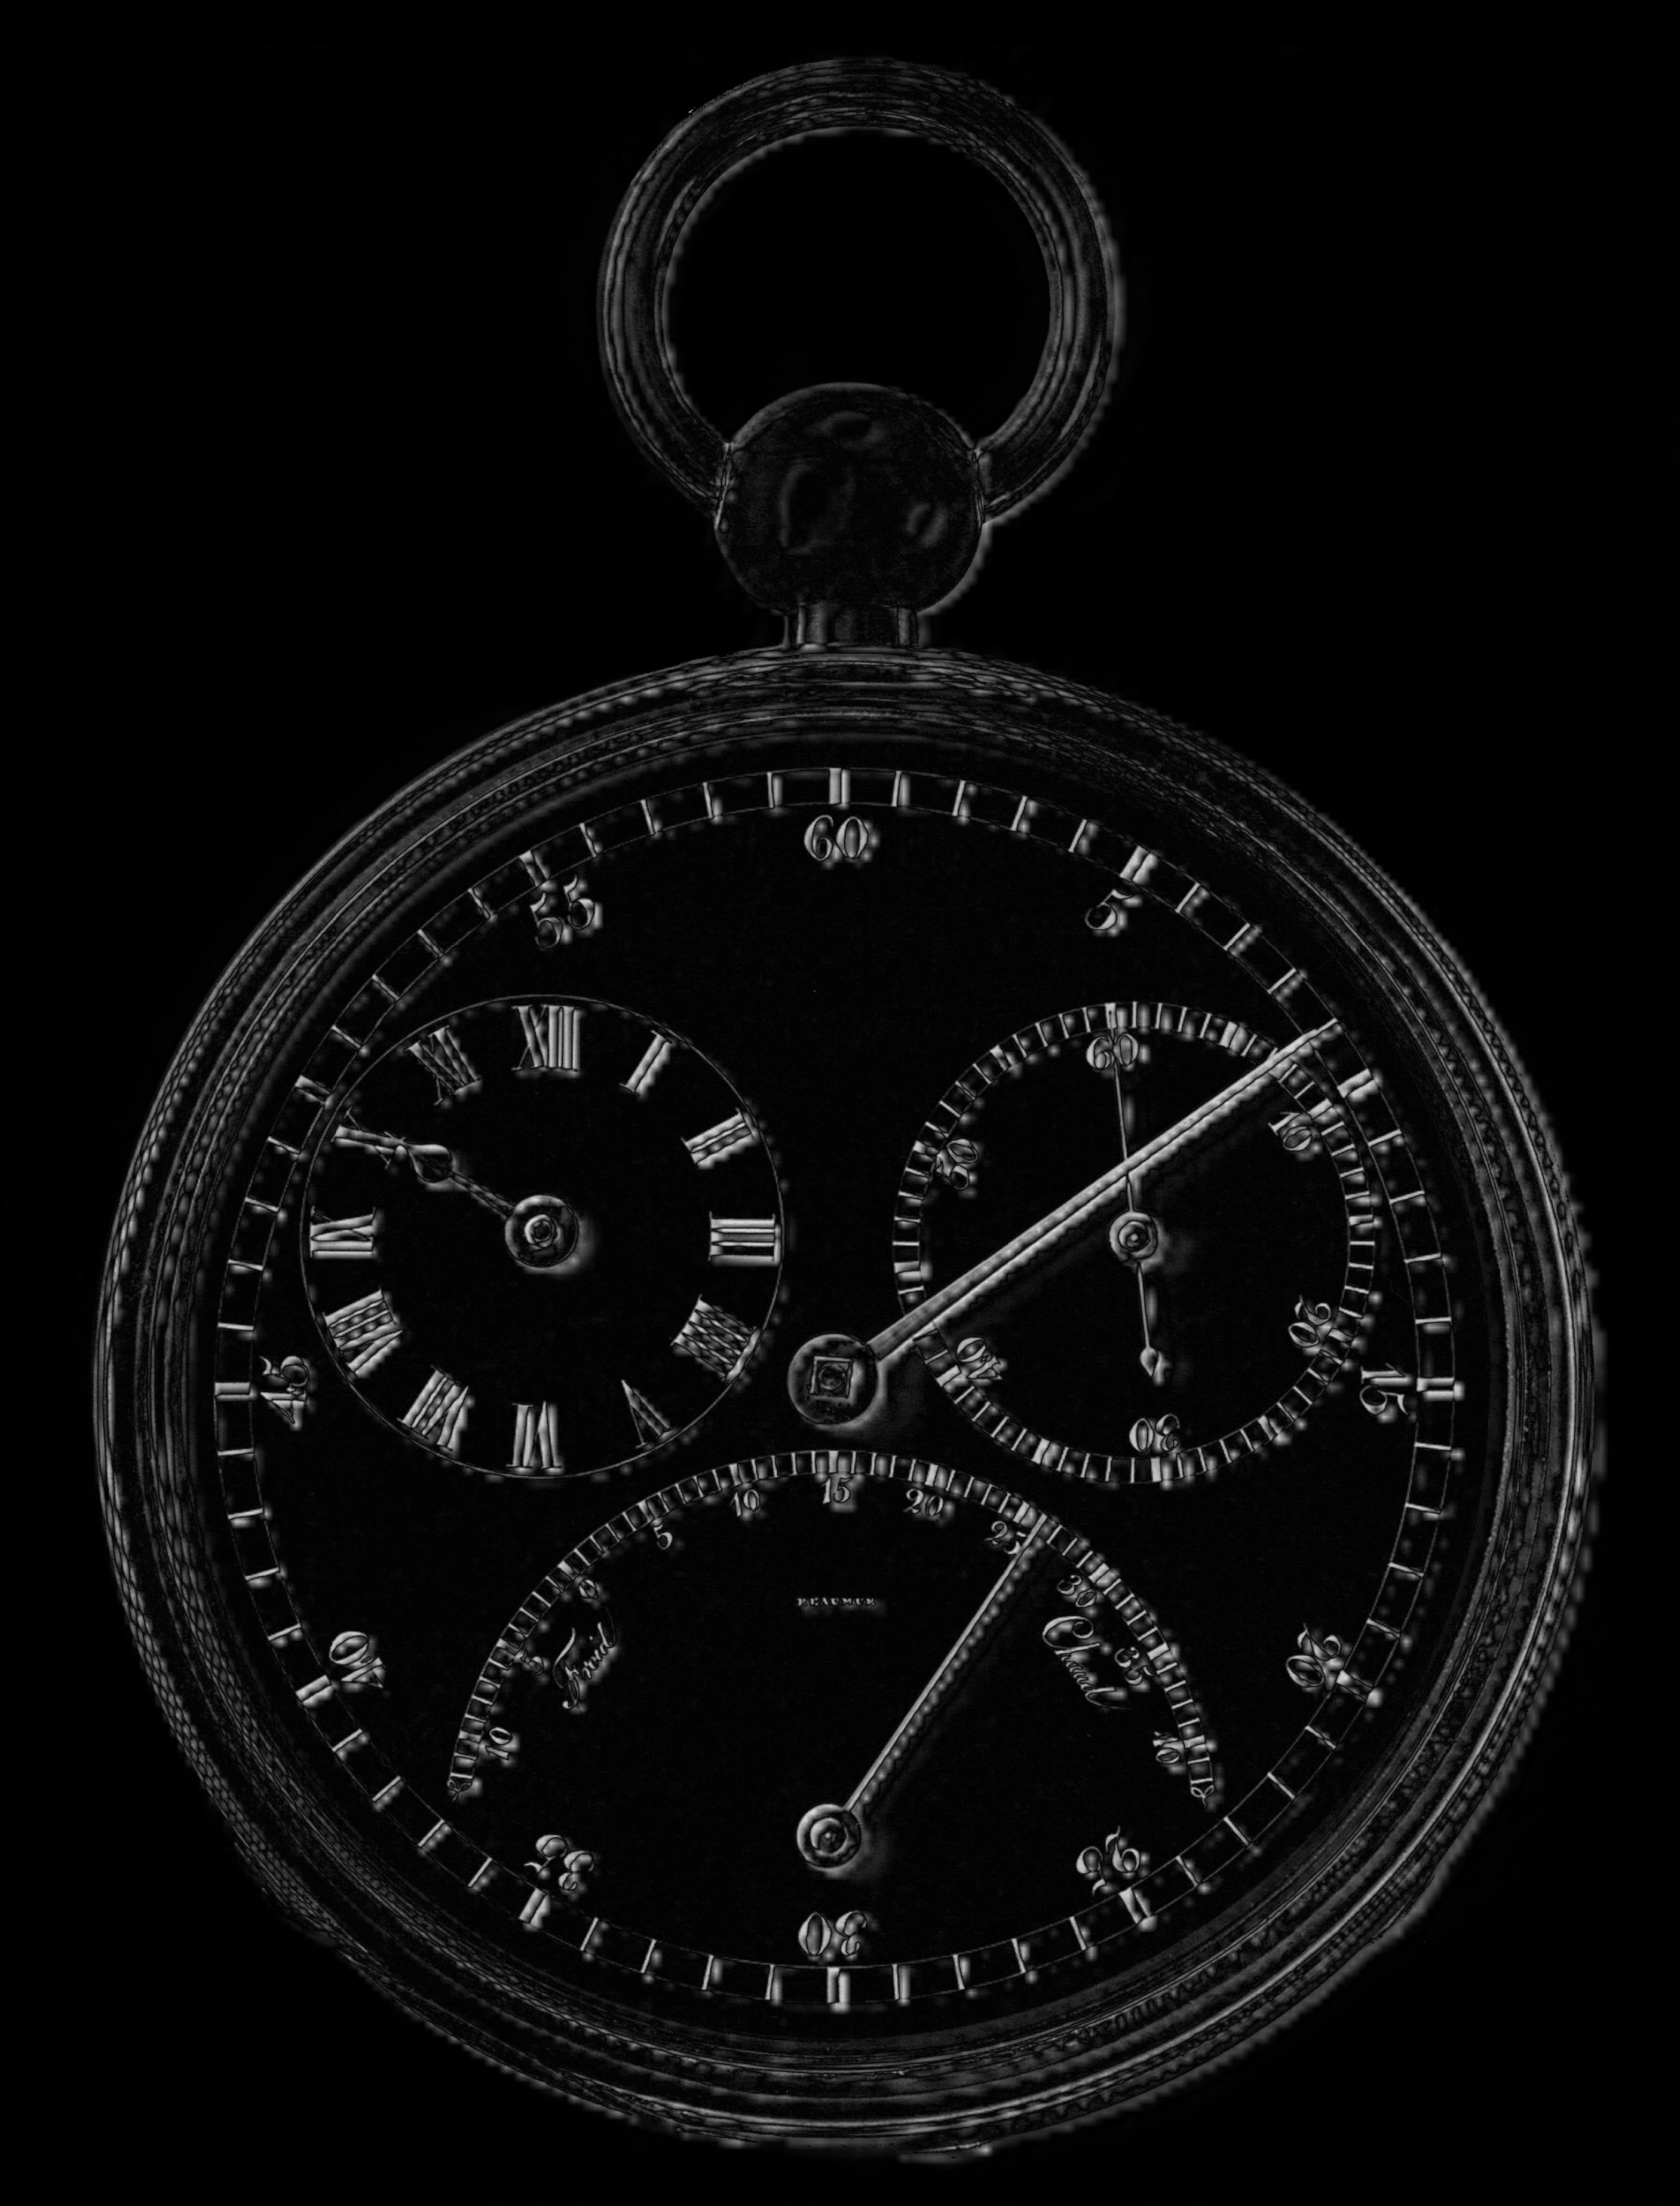
\includegraphics[width=\textwidth]{imgs/dif1.png}
        \caption{Imagem de diferença da imagem original (1250 dpi) com a de 300 dpi.}
        \label{fig:clock_original}
    \end{subfigure}%
    \hfill
    \begin{subfigure}[b]{0.3\textwidth}
        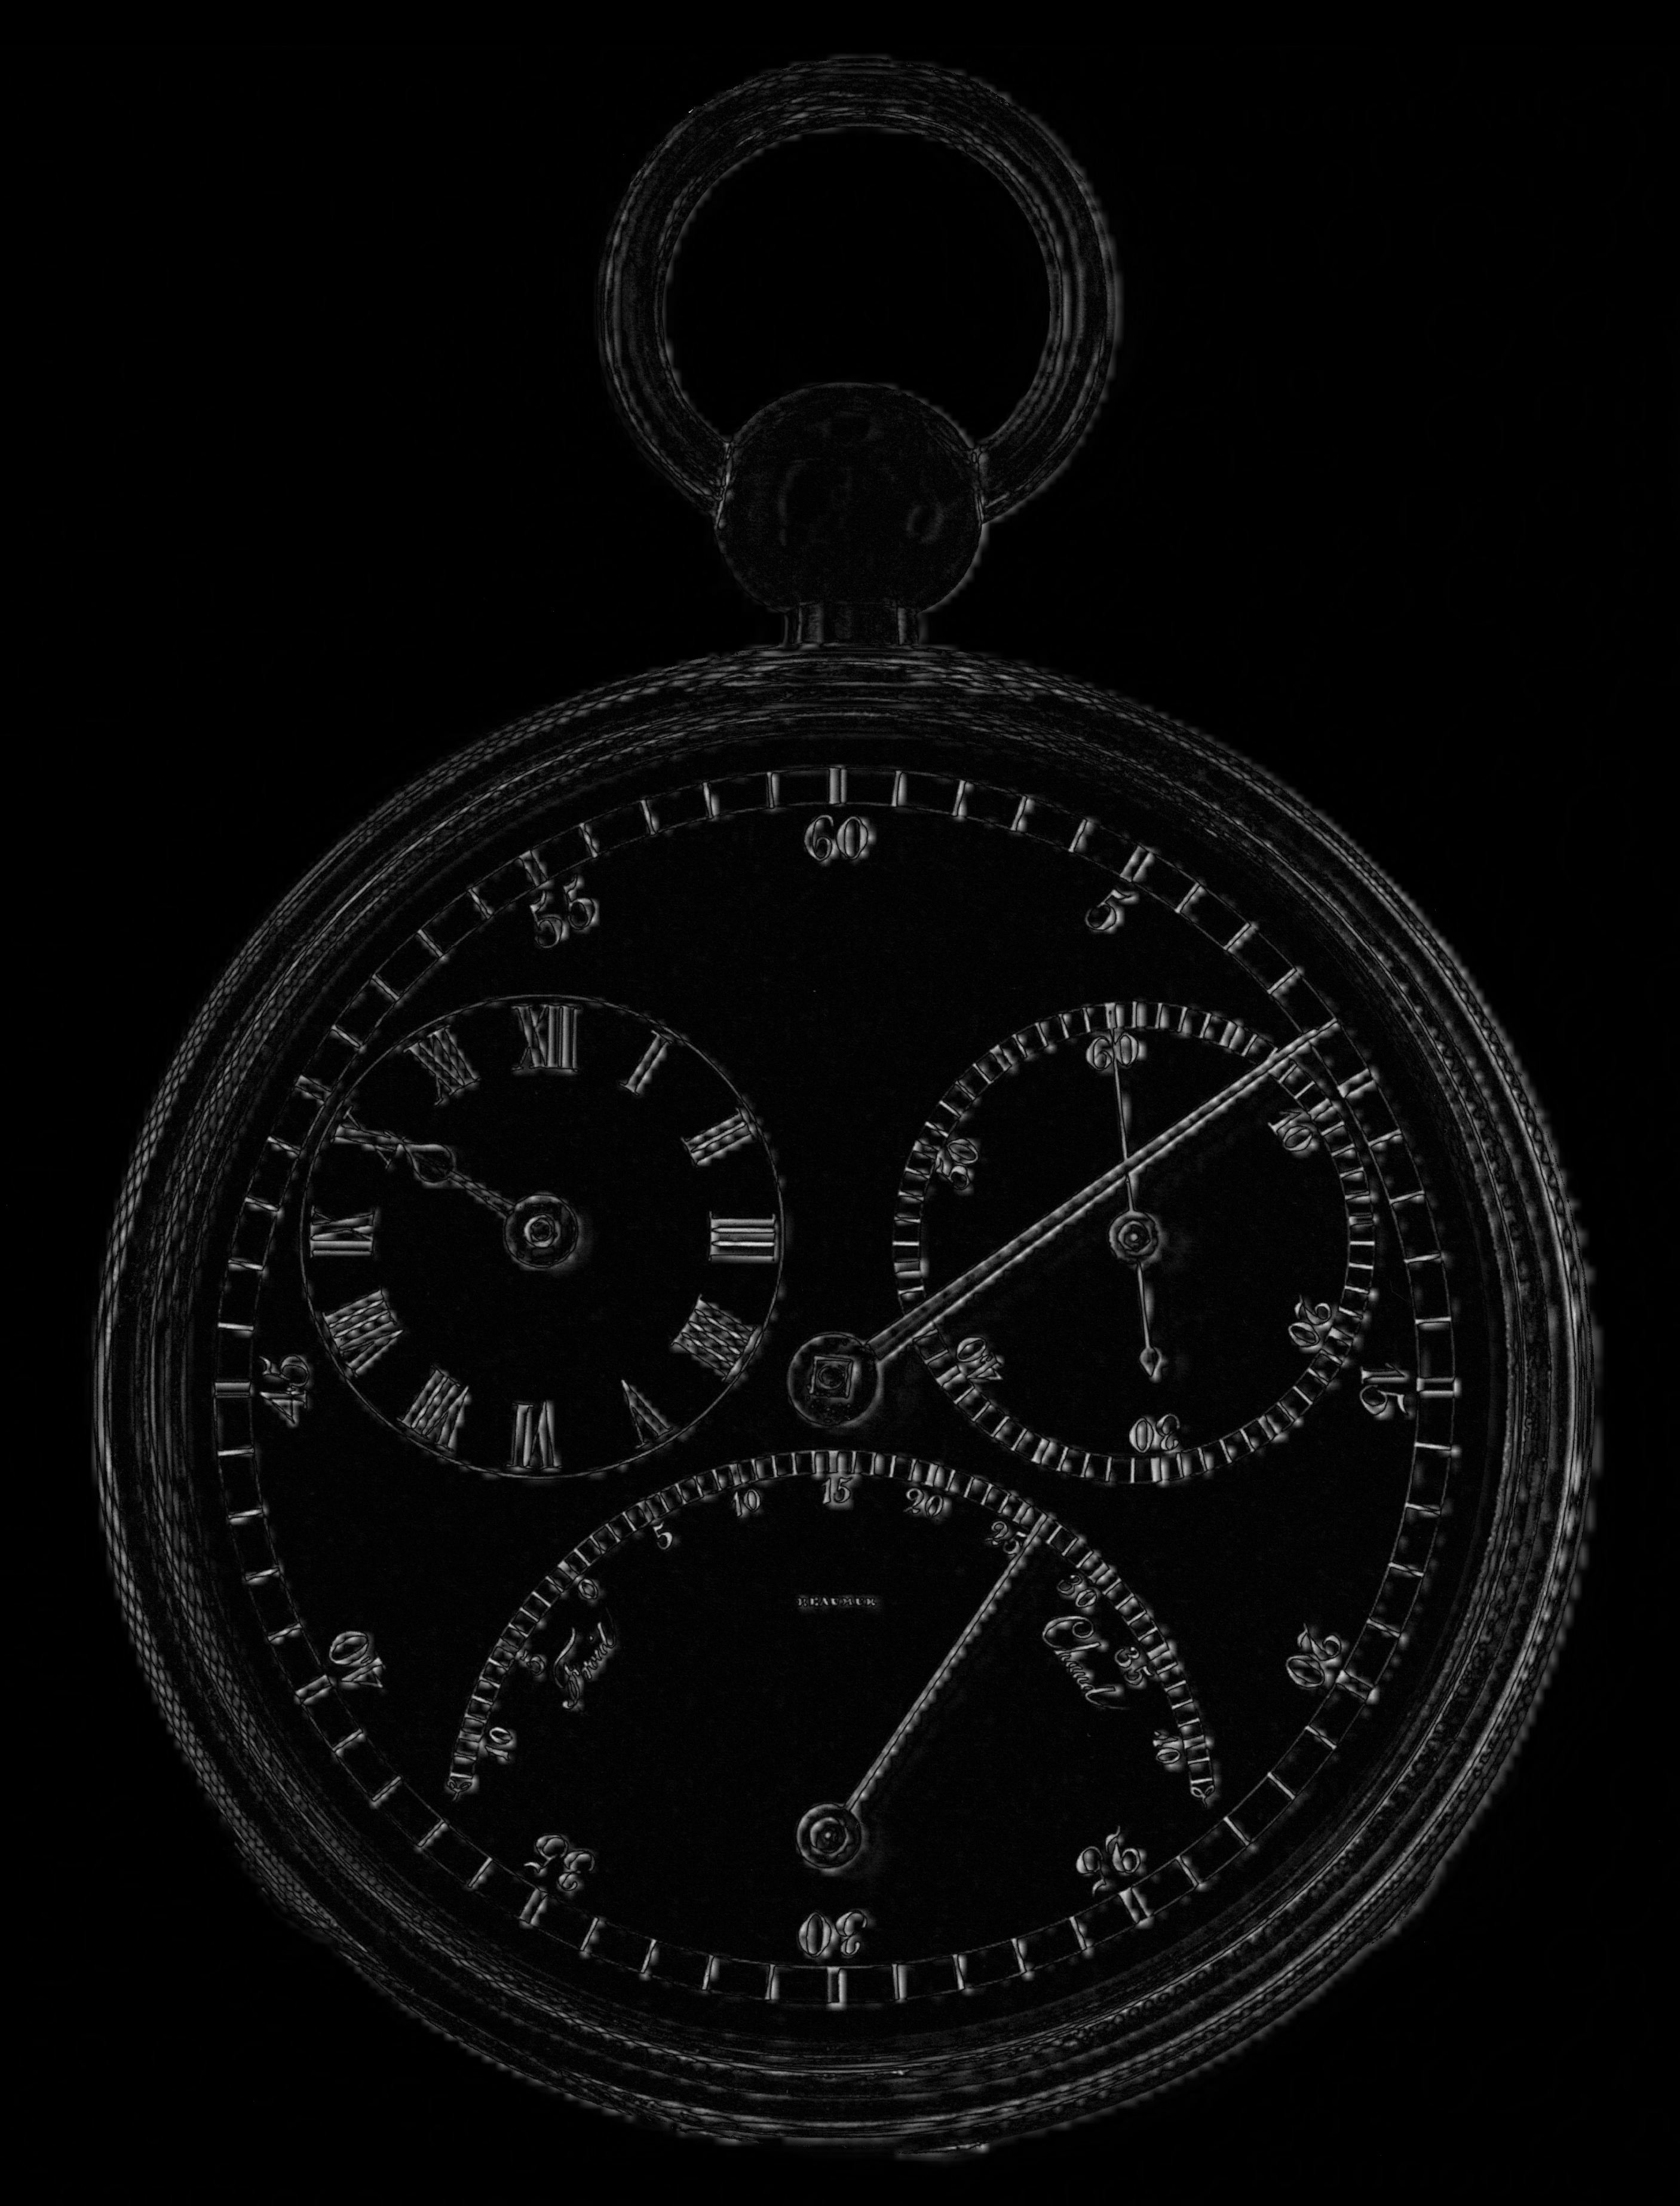
\includegraphics[width=\textwidth]{imgs/dif2.png}
        \caption{Imagem de diferença da imagem original (1250 dpi) com a de 1250 dpi interpolada.}
        \label{fig:clock_300dpi}
    \end{subfigure}%
    \label{fig:clock_comparison}
\end{figure}

Aplicamos o mesmo raciocínio a outras duas imagens escolhidas: imagem do coqueiro e imagem da chuva.

\begin{figure}[H]
    \centering
    \caption{Imagens do coqueiro.}
    \begin{subfigure}[b]{0.3\textwidth}
        \includegraphics[width=\textwidth]{imgs/2.1.png}
        \caption{Imagem original 300 dpi.}
    \end{subfigure}%
    \hfill
    \begin{subfigure}[b]{0.3\textwidth}
        \includegraphics[width=\textwidth]{imgs/2.2.png}
        \caption{Imagem modificada com 60 dpi.}
    \end{subfigure}%
    \hfill
    \begin{subfigure}[b]{0.3\textwidth}
        \includegraphics[width=\textwidth]{imgs/2.3.png}
        \caption{Imagem modificada com 300 dpi.}
    \end{subfigure}
    \hfill
    \caption{Imagens diferença do coqueiro.}
    \begin{subfigure}[b]{0.3\textwidth}
        \includegraphics[width=\textwidth]{imgs/dif2.1.png}
        \caption{Imagem de diferença da imagem original (300 dpi) com a de 60 dpi.}
    \end{subfigure}%
    \hfill
    \begin{subfigure}[b]{0.3\textwidth}
        \includegraphics[width=\textwidth]{imgs/dif2.2.png}
        \caption{Imagem de diferença da imagem original (300 dpi) com a de 300 dpi interpolada.}
    \end{subfigure}%
\end{figure}

\begin{figure}{H}
    \centering
    \caption{Imagens da chuva.}
    \begin{subfigure}[b]{0.3\textwidth}
        \includegraphics[width=\textwidth]{imgs/3.1.png}
        \caption{Imagem original 300 dpi.}
    \end{subfigure}%
    \hfill
    \begin{subfigure}[b]{0.3\textwidth}
        \includegraphics[width=\textwidth]{imgs/3.2.png}
        \caption{Imagem modificada com 60 dpi.}
    \end{subfigure}%
    \hfill
    \begin{subfigure}[b]{0.3\textwidth}
        \includegraphics[width=\textwidth]{imgs/3.3.png}
        \caption{Imagem modificada com 300 dpi.}
    \end{subfigure}
    \hfill
    \caption{Imagens diferença da chuva.}
    \begin{subfigure}[b]{0.3\textwidth}
        \includegraphics[width=\textwidth]{imgs/dif3.1.png}
        \caption{Imagem de diferença da imagem original (300 dpi) com a de 60 dpi.}

    \end{subfigure}%
    \hfill
    \begin{subfigure}[b]{0.3\textwidth}
        \includegraphics[width=\textwidth]{imgs/dif3.2.png}
        \caption{Imagem de diferença da imagem original (300 dpi) com a de 300 dpi interpolada.}
    \end{subfigure}%
\end{figure}
\vbox{} Conclui-se que, em determinadas condições, a interpolação bilinear é um ótimo método para interpolar pixels a uma imagem. Em especial, quando a diferença de intensidade entre pixels vizinhos é considerável, a interpolação é uma boa estratégia para aumentar a densidade de pixels (dpi). Além disso, por ser uma média ponderada, a interpolação bilinear acaba suavizando a diferença de intensidade entre pixels de uma imagem.
\section{Código Fonte em C++}
\lstinputlisting[language=C++, caption={Código fonte do programa de interpolação bilinear em C++.}]{main.cpp}
\lstinputlisting[language=C++, caption={Código fonte do programa de diferença de imagens em C++.}]{dif_tif.cpp}

\end{document}